% Options for packages loaded elsewhere
\PassOptionsToPackage{unicode}{hyperref}
\PassOptionsToPackage{hyphens}{url}
%
\documentclass[
]{article}
\usepackage{amsmath,amssymb}
\usepackage{iftex}
\ifPDFTeX
  \usepackage[T1]{fontenc}
  \usepackage[utf8]{inputenc}
  \usepackage{textcomp} % provide euro and other symbols
\else % if luatex or xetex
  \usepackage{unicode-math} % this also loads fontspec
  \defaultfontfeatures{Scale=MatchLowercase}
  \defaultfontfeatures[\rmfamily]{Ligatures=TeX,Scale=1}
\fi
\usepackage{lmodern}
\ifPDFTeX\else
  % xetex/luatex font selection
\fi
% Use upquote if available, for straight quotes in verbatim environments
\IfFileExists{upquote.sty}{\usepackage{upquote}}{}
\IfFileExists{microtype.sty}{% use microtype if available
  \usepackage[]{microtype}
  \UseMicrotypeSet[protrusion]{basicmath} % disable protrusion for tt fonts
}{}
\makeatletter
\@ifundefined{KOMAClassName}{% if non-KOMA class
  \IfFileExists{parskip.sty}{%
    \usepackage{parskip}
  }{% else
    \setlength{\parindent}{0pt}
    \setlength{\parskip}{6pt plus 2pt minus 1pt}}
}{% if KOMA class
  \KOMAoptions{parskip=half}}
\makeatother
\usepackage{xcolor}
\usepackage[margin=1in]{geometry}
\usepackage{graphicx}
\makeatletter
\def\maxwidth{\ifdim\Gin@nat@width>\linewidth\linewidth\else\Gin@nat@width\fi}
\def\maxheight{\ifdim\Gin@nat@height>\textheight\textheight\else\Gin@nat@height\fi}
\makeatother
% Scale images if necessary, so that they will not overflow the page
% margins by default, and it is still possible to overwrite the defaults
% using explicit options in \includegraphics[width, height, ...]{}
\setkeys{Gin}{width=\maxwidth,height=\maxheight,keepaspectratio}
% Set default figure placement to htbp
\makeatletter
\def\fps@figure{htbp}
\makeatother
\ifLuaTeX
  \usepackage{luacolor}
  \usepackage[soul]{lua-ul}
\else
  \usepackage{soul}
\fi
\setlength{\emergencystretch}{3em} % prevent overfull lines
\providecommand{\tightlist}{%
  \setlength{\itemsep}{0pt}\setlength{\parskip}{0pt}}
\setcounter{secnumdepth}{-\maxdimen} % remove section numbering
% definitions for citeproc citations
\NewDocumentCommand\citeproctext{}{}
\NewDocumentCommand\citeproc{mm}{%
  \begingroup\def\citeproctext{#2}\cite{#1}\endgroup}
\makeatletter
 % allow citations to break across lines
 \let\@cite@ofmt\@firstofone
 % avoid brackets around text for \cite:
 \def\@biblabel#1{}
 \def\@cite#1#2{{#1\if@tempswa , #2\fi}}
\makeatother
\newlength{\cslhangindent}
\setlength{\cslhangindent}{1.5em}
\newlength{\csllabelwidth}
\setlength{\csllabelwidth}{3em}
\newenvironment{CSLReferences}[2] % #1 hanging-indent, #2 entry-spacing
 {\begin{list}{}{%
  \setlength{\itemindent}{0pt}
  \setlength{\leftmargin}{0pt}
  \setlength{\parsep}{0pt}
  % turn on hanging indent if param 1 is 1
  \ifodd #1
   \setlength{\leftmargin}{\cslhangindent}
   \setlength{\itemindent}{-1\cslhangindent}
  \fi
  % set entry spacing
  \setlength{\itemsep}{#2\baselineskip}}}
 {\end{list}}
\usepackage{calc}
\newcommand{\CSLBlock}[1]{\hfill\break\parbox[t]{\linewidth}{\strut\ignorespaces#1\strut}}
\newcommand{\CSLLeftMargin}[1]{\parbox[t]{\csllabelwidth}{\strut#1\strut}}
\newcommand{\CSLRightInline}[1]{\parbox[t]{\linewidth - \csllabelwidth}{\strut#1\strut}}
\newcommand{\CSLIndent}[1]{\hspace{\cslhangindent}#1}
\usepackage{helvet}
\renewcommand*\familydefault{\sfdefault}
\usepackage{setspace}
\doublespacing
\usepackage[left]{lineno}
\linenumbers
\usepackage{booktabs}
\usepackage{longtable}
\usepackage{array}
\usepackage{multirow}
\usepackage{wrapfig}
\usepackage{float}
\usepackage{placeins}
\usepackage{colortbl}
\usepackage{pdflscape}
\usepackage{tabu}
\usepackage{threeparttable}
\usepackage{threeparttablex}
\usepackage[normalem]{ulem}
\usepackage{makecell}
\usepackage{xcolor}
\usepackage{caption}
\usepackage[labelformat=empty]{caption}
\usepackage{multirow}
\usepackage{multicol}
\usepackage{colortbl}
\usepackage{hhline}
\newlength\Oldarrayrulewidth
\newlength\Oldtabcolsep
\usepackage{longtable}
\usepackage{array}
\usepackage{hyperref}
\usepackage{float}
\usepackage{wrapfig}
\ifLuaTeX
  \usepackage{selnolig}  % disable illegal ligatures
\fi
\usepackage{bookmark}
\IfFileExists{xurl.sty}{\usepackage{xurl}}{} % add URL line breaks if available
\urlstyle{same}
\hypersetup{
  pdftitle={Transcriptomics of a THEV-infected Turkey B-cell Line},
  hidelinks,
  pdfcreator={LaTeX via pandoc}}

\title{Transcriptomics of a THEV-infected Turkey B-cell Line}
\author{}
\date{\vspace{-2.5em}}

\begin{document}
\maketitle

\vspace{5mm}

Abraham Quaye\({^\dagger}\)\textsuperscript{,a}, Brian D.
Poole\textsuperscript{a,*}

\vspace{5mm}

\textsuperscript{a}Department of Microbiology and Molecular Biology,
Brigham Young University\\
\({^\dagger}\)First-author\\
\textsuperscript{*}Corresponding Author

\vspace{5mm}

\textbf{Corresponding Author Information}\\
\href{mailto:brian_poole@byu.edu}{\nolinkurl{brian\_poole@byu.edu}}\\
Department of Microbiology and Molecular Biology,\\
4007 Life Sciences Building (LSB),\\
Brigham Young University,\\
Provo, Utah\\

\newpage

\subsection{ABSTRACT}\label{abstract}

\newpage

\subsection{INTRODUCTION}\label{introduction}

Turkey hemorrhagic enteritis virus (THEV), belonging to the family
\emph{Adenoviridae}, genus \emph{Siadenovirus}, infects turkeys,
chickens, and pheasants (1, 2). Infecting its hosts via the feco-oral
route, THEV causes hemorrhagic enteritis (HE) in turkeys, a debilitating
disease affecting predominantly 6-12 week old turkey poults
characterized by immunosuppression (IMS), depression, splenomegaly,
intestinal lesions leading to bloody droppings, and up to 80\% mortality
(3--6). The clinical disease usually persists in affected flocks for
about 7-10 days. However, secondary bacterial infections may extend the
duration of illness and mortality for an additional 2-3 weeks due to the
immunosuppressive nature of the virus, exacerbating the economic losses
(5, 7). Low pathogenic (avirulent) strains of THEV have been isolated,
which show subclinical infections but retain the immunosuppressive
effects. Since its isolation from a pheasant spleen, the Virginia
Avirulent Strain (VAS) has been used effectively as a live vaccine
despite the immunosuppressive side-effects but the vaccinated birds are
rendered more susceptible to opportunistic infections and death than
unvaccinated cohorts leading to significant economic losses (4, 5,
8--10).

It is well-established that THEV primarily infects and replicates in
turkey B-cells of the bursa and spleen and somewhat in macrophages,
inducing apoptosis and necrosis. Consequently, a significant drop in
number of B-cells (specifically, IgM+ B-cells) and macrophages ensue
along with increased T-cell counts with abnormal T-cell subpopulation
(CD4+ and CD8+) ratios. The cell death seen in the B-cells and
macrophages is generally proposed as the major cause of THEV-induced IMS
as both humoral and cell-mediated immunity are impaired (5, 6, 8, 11).
It is also thought that the virus replication in the spleen attracts
T-cells and peripheral blood macrophages to the spleen where the T-cells
are activated by cytokines from activated macrophages and vice versa.
The activated T-cells undergo clonal expansion and secrete interferons:
type I (IFN-\(\alpha\) and IFN-\(\beta\)) and type II (IFN-\(\gamma\))
as well as tumor necrosis factor (TNF) while activated macrophages
secrete interleukin 6 (IL-6), TNF, and nitric oxide (NO), an antiviral
agent with immunosuppressive properties. The inflammatory cytokines
released by T-cells and macrophages (e.g., TNF and IL-6) may also induce
apoptosis in bystander splenocytes, exacerbating the already numerous
apoptotic and necrotic splenocytes, culminating in IMS (8, 11) (see
\textbf{Figure 1}). However, the precise molecular mechanisms of
THEV-induced IMS or pathways involved are poorly understood (6).
Elucidating the specific mechanisms and pathways of THEV-induced IMS is
the most crucial step in THEV research as it will present a means of
mitigating the IMS.

Next generation sequencing (NGS) is a groundbreaking technology that has
significantly enhanced our understanding of DNA and RNA structure and
function, and facilitated exceptional advancements in all domains of
biology and the Life Sciences, including studies in rare genetic
diseases, cancer genomics, microbiome analysis, infectious diseases, and
population genetics (12). mRNA sequencing (RNA-seq), an NGS approach to
transcriptomic studies, is a versatile, high throughput, and
cost-effective technology that allows a broad scan of the entire
transcriptome (the complete set of RNA molecules produced under specific
conditions or in specific cells), thereby uncovering the active genes
and molecular pathways and processes. This technology has been leveraged
in uncountable number of studies to elucidate active cellular processes
under a wide range of treatment conditions, including the
transcriptomics of viral infections (12--16). In RNA-seq studies,
differentially expressed genes (DEGs) identified under different
experimental conditions are key to unlocking the interesting biology or
mechanism under study. Identified DEGs are typically used for functional
enrichment analysis in large curated knowledgebases which connect genes
to specific biological processes, functions, and pathways such as gene
ontology (GO) and Kyoto Encyclopedia of Genes and Genomes (KEGG)
pathways, shedding light on the biological question under study (17,
18).

To the best of our knowledge, no study has leveraged the wealth of
information offered by RNA-seq to elucidate the molecular mechanisms and
pathways leading to THEV-induced IMS. To effectively counteract the
immunosupressive effect of the vaccine, it is essential to unravel the
host mechanisms/pathways influenced by the virus to bring about IMS. In
this study, we present the first transcriptomic profile of a THEV
infection using paired-end RNA-seq in a turkey B-cell line (MDTC-RP19),
highlighting key host genes, cellular/molecular processes and pathways
affected during a THEV infection. Our RNA-seq yielded 149 bp long high
quality (mean PHRED Score of 36) sequences from each end of cDNA
fragments, which were mapped to the genome of domestic turkey
(\emph{Meleagris gallopavo}). \newpage

\subsection{RESULTS}\label{results}

\textbf{Sequencing Results}\\
To identify the host transcriptome profile of THEV infection, MDTC-RP19
cells were THEV-infected or mock-infected in triplicates or duplicates,
respectively, and collected in like manner at 4-, 12-, 24-, and 72-hours
post infection (hpi). mRNAs extracted from mock- or THEV-infected cells
in duplicates or triplicates, respectively, were sequenced on the
Illumina platform. The sequencing yielded a total of \textbf{776.1}
million raw reads (149 bp in length) across all samples (statistics for
the sequencing reads obtained from each RNA library are presented in
\textbf{Table 1}). After trimming off low-quality reads, the remaining
\textbf{742.8} million total paired-end trimmed reads (approximately,
\textbf{34.7}-\textbf{47.9} million reads per sample) were mapped to the
genome of \emph{Meleagris gallopavo} obtained from the National Center
for Biotechnology Information (NCBI). The percentage of reads mapping to
the host genome across all samples ranged from
\textbf{32.4}-\textbf{89.2}\%. Although our sequencing reads have
excellent quality scores (see \textbf{Table 1}) for all time points, the
DEGs identified at 4- and 72-hpi did not yield any results in the
functional enrichment analyses (i.e, GO term and KEGG pathway); hence,
they were excluded from all subsequent analyses.

\textbf{DEGs of Infected Versus Mock-infected Cells}\\
\st{Discuss selection criteria and method/software used}\\
\st{Number of DEGs}\\
\st{Discuss all the QC plots (volcano, sample corr, pca, etc.) here}\\
\st{Discuss fold changes?}

\textbf{Functional Enrichment Analyses (GO, KEGG pathway, and
interaction network analyses)}\\
\st{Discuss enrichment analysis plots and tables here} \newpage

\subsection{DISCUSSION}\label{discussion}

\newpage

\subsection{CONCLUSIONS}\label{conclusions}

\newpage

\subsection{MATERIALS AND METHODS}\label{materials-and-methods}

\textbf{Cell culture and THEV Infection}\\
The Turkey B-cell line (MDTC-RP19, ATCC CRL-8135) was grown as
suspension cultures in 1:1 complete Leibovitz's L-15/McCoy's 5A medium
with 10\% fetal bovine serum (FBS), 20\% chicken serum (ChS), 5\%
tryptose phosphate broth (TPB), and 1\% antibiotic solution (100 U/mL
Penicillin and 100\(\mu g\)/mL Streptomycin), at 41\textsuperscript{o}C
in a humidified atmosphere with 5\% CO\textsubscript{2}. Infected cells
were maintained in 1:1 serum-reduced Leibovitz's L15/McCoy's 5A media
(SRLM) with 2.5\% FBS, 5\% ChS, 1.2\% TPB, and 1\% antibiotic solution.
A commercially available THEV vaccine was purchased from Hygieia
Biological Labs (VAS strain). The stock virus was titrated using an
in-house qPCR assay with titer expressed as genome copy number (GCN)/mL,
similar to Mahshoub \emph{et al} (19) with modifications. Cells were
THEV-infected or mock-infected in triplicates or duplicates,
respectively at a multiplicity of infection (MOI) of 100 GCN/cell,
incubated at 41\textsuperscript{o}C for 1 hour, and washed three times
with phosphate buffered saline (PBS) to get rid of free virus particles.
At each time point (4-, 12-, 24-, and 72-hpi), triplicate
(THEV-infected) and duplicate (mock-infected) samples were harvested for
total RNA extraction.

\textbf{RNA extraction and Sequencing}\\
Total RNA was extracted from infected cells using the Thermofisher
RNAqueous™-4PCR Total RNA Isolation Kit (which includes a DNase I
digestion step) per manufacturer's instructions. An agarose gel
electrophoresis was performed to check RNA integrity. The RNA quantity
and purity was initially assessed using nanodrop, and RNA was used only
if the A260/A280 ratio was 2.0 ± 0.05 and the A260/A230 ratio was
\textgreater2 and \textless2.2. Extracted total RNA samples were sent to
LC Sciences, Houston TX for poly-A-tailed mRNA sequencing where RNA
integrity was checked with Agilent Technologies 2100 Bioanalyzer High
Sensitivity DNA Chip and poly(A) RNA-seq library was prepared following
Illumina's TruSeq-stranded-mRNA sample preparation protocol. Paired-end
sequencing, generating 150 bp reads was performed on the Illumina
NovaSeq 6000 sequencing system. The paired-end 150bp sequences obtained
during this study and all expression data have been submitted to the
Gene Expression Omnibus database, under accession no \#\#\#\#\#\#\#

\textbf{Quality Control and Mapping Process}\\
Sequencing reads were processed following a well-established protocol
described by Pertea \emph{et al} (20), using Snakemake - version 7.32.4
(21), a popular workflow management system to drive the pipeline.
Briefly, raw sequencing reads were trimmed with Cutadapt - version 1.10
(22) and the quality of trimmed reads evaluated using the FastQC
software, version 0.12.1 (Bioinformatics Group at the Babraham
Institute, Cambridge, United Kingdom;
www.bioinformatics.babraham.ac.uk), achieving an overall Mean Sequence
Quality (PHRED Score) of 36. Trimmed reads were mapped the reference
\emph{Meleagris gallopavo} genome
(\url{https://ftp.ncbi.nlm.nih.gov/genomes/all/GCF/000/146/605/GCF_000146605.3_Turkey_5.1/GCF_000146605.3_Turkey_5.1_genomic.fna.gz})
with Hisat2 - version 2.2.1 (20) using the accompanying gene transfer
format (GTF) annotation file
(\url{https://ftp.ncbi.nlm.nih.gov/genomes/all/GCF/000/146/605/GCF_000146605.3_Turkey_5.1/GCF_000146605.3_Turkey_5.1_genomic.gtf.gz})
to build a genomic index. Samtools - version 1.19.2 was used to convert
the output Sequence Alignment Map (SAM) file to the more manageable
Binary Alignment Map (BAM) format. The StringTie (v2.2.1) software (20),
set to expression estimation mode was used to generate normalized gene
expression estimates from the BAM files for genes in the reference GTF
file after which the prepDE.py3 script was used to extract read count
information from the StringTie gene expression files, providing an
expression-count matrix for downstream DEG analysis.

\textbf{DEG Analysis and Functional Enrichment Analysis}\\
DEG analysis between mock- and THEV-infected samples was performed using
the very popular DESeq2 (23), which employs a Negative Binomial
distribution model for read count comparisons. Genes with
P\textsubscript{adjusted}-value \(\leq\) 0.05 were considered as
differentially expressed. The read count data are deposited at Gene
Expression Omnibus (GEO) under accession number \#\#\#. GO and KEGG
analyses for DEGs were performed based on GO databases and KEGG
databases using the R package gprofiler2 (24) with \emph{Meleagris
gallopavo} as the reference organism. Results with
P\textsubscript{adjusted}-value \(\leq\) 0.05 were included as
functionally enriched. \st{Additionally, the DAVID analysis tool was
used for KEGG pathway analysis}. All visualization plots were made using
ggplot2, pheatmap, and ggvenn R packages (25--27). Venn diagram ---

\textbf{Validation of DEGs by Reverse Transcriptase Quantitative PCR
(RT-qPCR)}

\textbf{Statistical Analysis} \newpage

\subsection{DATA AVAILABILITY}\label{data-availability}

\newpage

\subsection{CODE AVAILABILITY}\label{code-availability}

\newpage

\subsection{ACKNOWLEDGMENTS}\label{acknowledgments}

\newpage

\subsection{REFERENCES}\label{references}

\setlength{\parindent}{-0.25in}
\setlength{\leftskip}{0.25in}

\noindent

\phantomsection\label{refs}
\begin{CSLReferences}{0}{1}
\bibitem[\citeproctext]{ref-Harrach2008}
\CSLLeftMargin{1. }%
\CSLRightInline{Harrach B. 2008.
\href{https://doi.org/10.1016/B978-012374410-4.00680-4}{Adenoviruses:
General features}, p. 1--9. \emph{In} Mahy, BWJ, Van Regenmortel, MHV
(eds.), Encyclopedia of virology (third edition). Book Section. Academic
Press, Oxford.}

\bibitem[\citeproctext]{ref-Davison2003}
\CSLLeftMargin{2. }%
\CSLRightInline{Davison A, Benko M, Harrach B. 2003.
\href{https://doi.org/10.1099/vir.0.19497-0}{Genetic content and
evolution of adenoviruses}. The Journal of general virology
84:2895--908.}

\bibitem[\citeproctext]{ref-Gross1967}
\CSLLeftMargin{3. }%
\CSLRightInline{Gross WB, Moore WE. 1967. Hemorrhagic enteritis of
turkeys. Avian Dis 11:296--307.}

\bibitem[\citeproctext]{ref-Beach2006}
\CSLLeftMargin{4. }%
\CSLRightInline{Beach NM. 2006.
\href{http://scholar.lib.vt.edu/theses/available/etd-08142006-145339/}{Characterization
of avirulent turkey hemorrhagic enteritis virus: A study of the
molecular basis for variation in virulence and the occurrence of
persistent infection}. Thesis.}

\bibitem[\citeproctext]{ref-Dhama2017}
\CSLLeftMargin{5. }%
\CSLRightInline{Dhama K, Gowthaman V, Karthik K, Tiwari R, Sachan S,
Kumar MA, Palanivelu M, Malik YS, Singh RK, Munir M. 2017.
\href{https://doi.org/10.1080/01652176.2016.1277281}{Haemorrhagic
enteritis of turkeys -- current knowledge}. Veterinary Quarterly
37:31--42.}

\bibitem[\citeproctext]{ref-Tykaowski2019}
\CSLLeftMargin{6. }%
\CSLRightInline{Tykałowski B, Śmiałek M, Koncicki A, Ognik K, Zduńczyk
Z, Jankowski J. 2019.
\href{https://doi.org/10.1186/s12917-019-2138-8}{The immune response of
young turkeys to haemorrhagic enteritis virus infection at different
levels and sources of methionine in the diet}. BMC Veterinary Research
15.}

\bibitem[\citeproctext]{ref-Pierson2008}
\CSLLeftMargin{7. }%
\CSLRightInline{Pierson F, Fitzgerald S. 2008. Hemorrhagic enteritis and
related infections. Diseases of Poultry 276--286.}

\bibitem[\citeproctext]{ref-Rautenschlein2000}
\CSLLeftMargin{8. }%
\CSLRightInline{Rautenschlein S, Sharma JM. 2000.
\href{https://doi.org/10.1016/s0145-305x(99)00075-0}{Immunopathogenesis
of haemorrhagic enteritis virus (HEV) in turkeys}. Dev Comp Immunol
24:237--46.}

\bibitem[\citeproctext]{ref-Larsen1985}
\CSLLeftMargin{9. }%
\CSLRightInline{Larsen CT, Domermuth CH, Sponenberg DP, Gross WB. 1985.
Colibacillosis of turkeys exacerbated by hemorrhagic enteritis virus.
Laboratory studies. Avian Dis 29:729--32.}

\bibitem[\citeproctext]{ref-Beach2009a}
\CSLLeftMargin{10. }%
\CSLRightInline{Beach NM, Duncan RB, Larsen CT, Meng XJ, Sriranganathan
N, Pierson FW. 2009.
\href{https://doi.org/10.1637/8575-010509-reg.1}{Persistent infection of
turkeys with an avirulent strain of turkey hemorrhagic enteritis virus}.
Avian Diseases 53:370--375.}

\bibitem[\citeproctext]{ref-Rautenschlein2000b}
\CSLLeftMargin{11. }%
\CSLRightInline{Rautenschlein S, Suresh M, Sharma JM. 2000.
\href{https://doi.org/10.1007/s007050070083}{Pathogenic avian adenovirus
type II induces apoptosis in turkey spleen cells}. Archives of Virology
145:1671--1683.}

\bibitem[\citeproctext]{ref-Satam2023}
\CSLLeftMargin{12. }%
\CSLRightInline{Satam H, Joshi K, Mangrolia U, Waghoo S, Zaidi G, Rawool
S, Thakare RP, Banday S, Mishra AK, Das G, Malonia SK. 2023.
\href{https://doi.org/10.3390/biology12070997}{Next-generation
sequencing technology: Current trends and advancements}. Biology
12:997.}

\bibitem[\citeproctext]{ref-Pandey2023}
\CSLLeftMargin{13. }%
\CSLRightInline{Pandey D, Onkara Perumal P. 2023.
\href{https://doi.org/10.1007/s10142-023-01064-6}{A scoping review on
deep learning for next-generation RNA-seq. Data analysis}. Functional
\&amp; Integrative Genomics 23.}

\bibitem[\citeproctext]{ref-Wang2019}
\CSLLeftMargin{14. }%
\CSLRightInline{Wang B, Kumar V, Olson A, Ware D. 2019.
\href{https://doi.org/10.3389/fgene.2019.00384}{Reviving the
transcriptome studies: An insight into the emergence of single-molecule
transcriptome sequencing}. Frontiers in Genetics 10.}

\bibitem[\citeproctext]{ref-Choi2016}
\CSLLeftMargin{15. }%
\CSLRightInline{Choi SC. 2016.
\href{https://doi.org/10.1007/s12275-016-6233-2}{On the study of
microbial transcriptomes using second- and third-generation sequencing
technologies}. Journal of Microbiology 54:527--536.}

\bibitem[\citeproctext]{ref-Mo2023}
\CSLLeftMargin{16. }%
\CSLRightInline{Mo Q, Feng K, Dai S, Wu Q, Zhang Z, Ali A, Deng F, Wang
H, Ning Y-J. 2023.
\href{https://doi.org/10.1016/j.virs.2022.09.002}{Transcriptome
profiling highlights regulated biological processes and type III
interferon antiviral responses upon crimean-congo hemorrhagic fever
virus infection}. Virologica Sinica 38:34--46.}

\bibitem[\citeproctext]{ref-Ashburner2000}
\CSLLeftMargin{17. }%
\CSLRightInline{Ashburner M, Ball CA, Blake JA, Botstein D, Butler H,
Cherry JM, Davis AP, Dolinski K, Dwight SS, Eppig JT, Harris MA, Hill
DP, Issel-Tarver L, Kasarskis A, Lewis S, Matese JC, Richardson JE,
Ringwald M, Rubin GM, Sherlock G. 2000.
\href{https://doi.org/10.1038/75556}{Gene ontology: Tool for the
unification of biology}. Nature Genetics 25:25--29.}

\bibitem[\citeproctext]{ref-Kanehisa2000}
\CSLLeftMargin{18. }%
\CSLRightInline{Kanehisa M. 2000.
\href{https://doi.org/10.1093/nar/28.1.27}{KEGG: Kyoto encyclopedia of
genes and genomes}. Nucleic Acids Research 28:27--30.}

\bibitem[\citeproctext]{ref-Mahsoub2017}
\CSLLeftMargin{19. }%
\CSLRightInline{Mahsoub HM, Evans NP, Beach NM, Yuan L, Zimmerman K,
Pierson FW. 2017.
\href{https://doi.org/10.1016/j.jviromet.2016.11.002}{Real-time
{PCR}-based infectivity assay for the titration of turkey hemorrhagic
enteritis virus, an adenovirus, in live vaccines}. Journal of
Virological Methods 239:42--49.}

\bibitem[\citeproctext]{ref-Pertea2016}
\CSLLeftMargin{20. }%
\CSLRightInline{Pertea M, Kim D, Pertea GM, Leek JT, Salzberg SL. 2016.
\href{https://doi.org/10.1038/nprot.2016.095}{Transcript-level
expression analysis of RNA-seq experiments with HISAT, StringTie and
ballgown}. Nature Protocols 11:1650--1667.}

\bibitem[\citeproctext]{ref-Snakemake2021}
\CSLLeftMargin{21. }%
\CSLRightInline{Mölder F, Jablonski KP, Letcher B, Hall MB,
Tomkins-Tinch CH, Sochat V, Forster J, Lee S, Twardziok SO, Kanitz A,
Wilm A, Holtgrewe M, Rahmann S, Nahnsen S, Köster J. 2021.
\href{https://doi.org/10.12688/f1000research.29032.2}{Sustainable data
analysis with snakemake}. F1000Research 10:33.}

\bibitem[\citeproctext]{ref-Martin2011}
\CSLLeftMargin{22. }%
\CSLRightInline{Martin M. 2011.
\href{https://doi.org/10.14806/ej.17.1.200}{Cutadapt removes adapter
sequences from high-throughput sequencing reads}. EMBnetjournal 17:10.}

\bibitem[\citeproctext]{ref-Deseq2}
\CSLLeftMargin{23. }%
\CSLRightInline{Love MI, Huber W, Anders S. 2014.
\href{https://doi.org/10.1186/s13059-014-0550-8}{Moderated estimation of
fold change and dispersion for RNA-seq data with DESeq2}. Genome Biology
15:550.}

\bibitem[\citeproctext]{ref-Gprofiler2}
\CSLLeftMargin{24. }%
\CSLRightInline{Kolberg L, Raudvere U, Kuzmin I, Vilo J, Peterson H.
2020. gprofiler2-- an r package for gene list functional enrichment
analysis and namespace conversion toolset g:profiler. F1000Research 9
(ELIXIR).}

\bibitem[\citeproctext]{ref-ggplot2}
\CSLLeftMargin{25. }%
\CSLRightInline{Wickham H. 2016. ggplot2: Elegant graphics for data
analysis. Springer-Verlag New York.
\url{https://ggplot2.tidyverse.org}.}

\bibitem[\citeproctext]{ref-pheatmap}
\CSLLeftMargin{26. }%
\CSLRightInline{Kolde R. 2019. Pheatmap: Pretty heatmaps.
\url{https://CRAN.R-project.org/package=pheatmap}.}

\bibitem[\citeproctext]{ref-ggvenn}
\CSLLeftMargin{27. }%
\CSLRightInline{Yan L. 2023. Ggvenn: Draw venn diagram by 'ggplot2'.
\url{https://CRAN.R-project.org/package=ggvenn}.}

\end{CSLReferences}

\setlength{\parindent}{0in}
\setlength{\leftskip}{0in}
\newpage

\newpage

\subsection{TABLES AND FIGURES}\label{tables-and-figures}

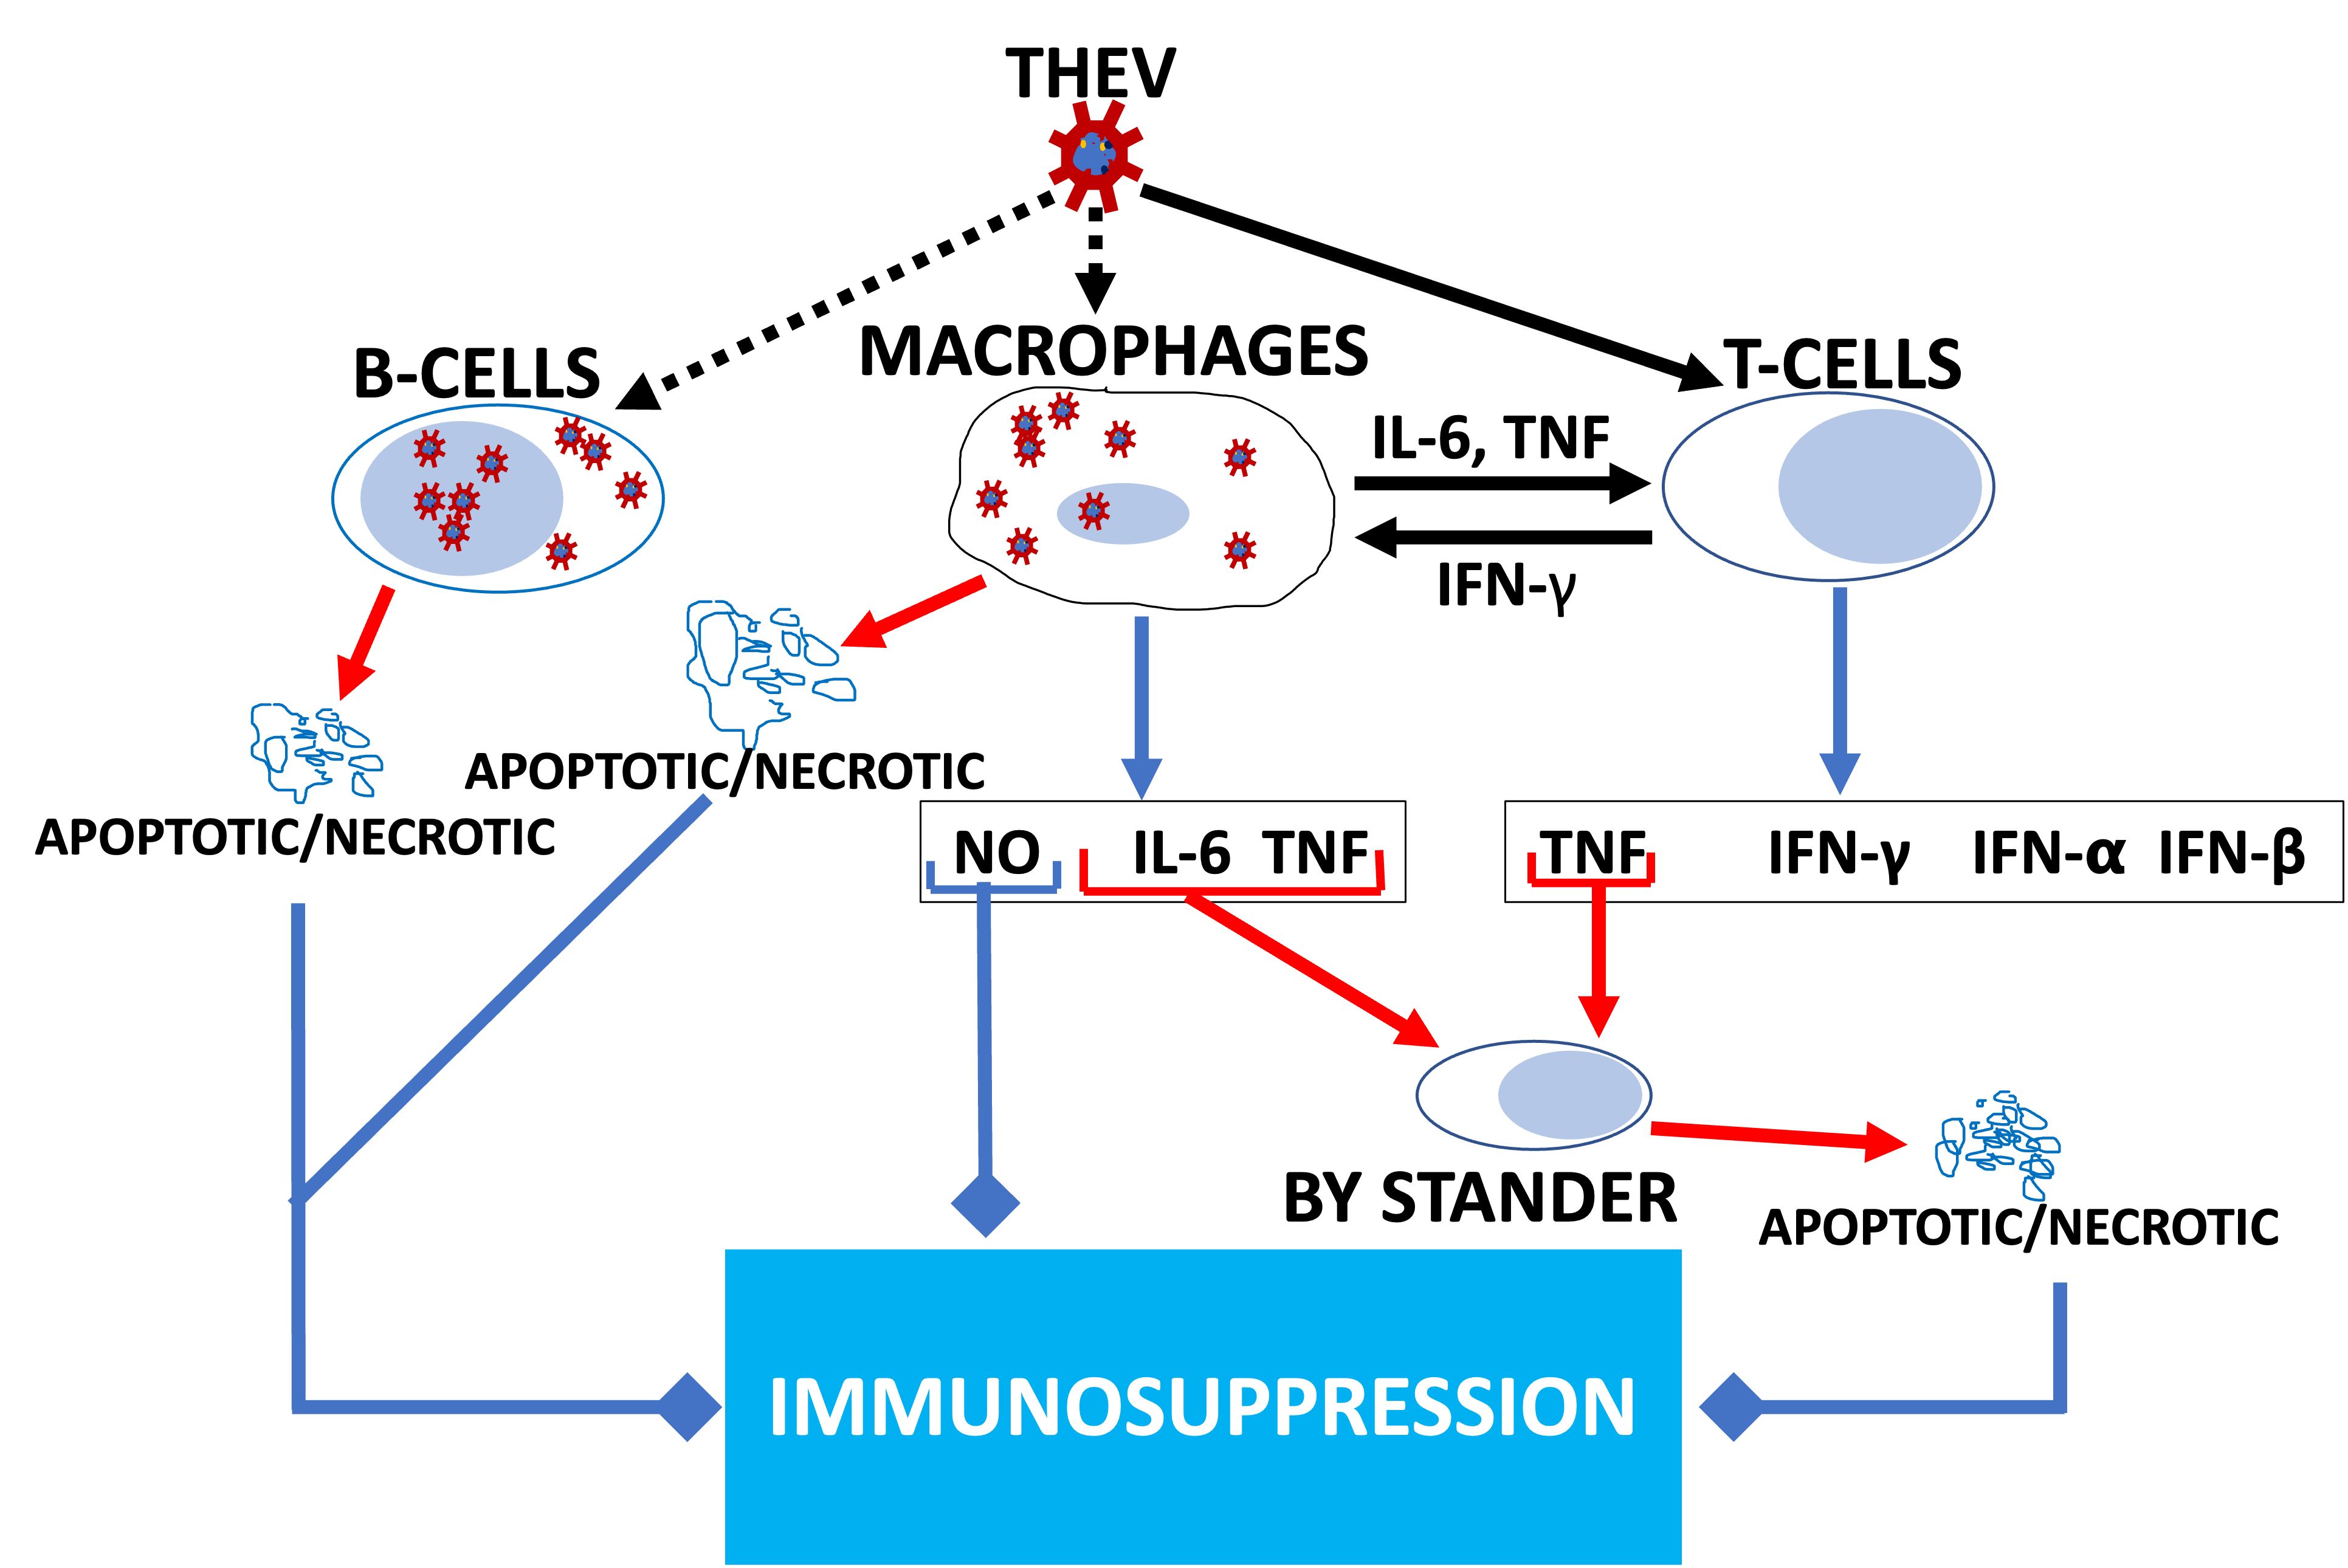
\includegraphics{results/imss_model.png} \textbf{Figure 1: Model of
THEV-induced immunosuppression in turkeys}. THEV infection of target
cells is indicated with black dotted arrows. Black unbroken arrows
indicate cell activation. Red arrows indicated signals leading to
apoptosis. Blue arrows indicate all cytokines released by the cell. Blue
arrows with square heads indicated an event leading to IMS. Adapted from
((8)) \newpage

\global\setlength{\Oldarrayrulewidth}{\arrayrulewidth}

\global\setlength{\Oldtabcolsep}{\tabcolsep}

\setlength{\tabcolsep}{2pt}

\renewcommand*{\arraystretch}{1.5}



\providecommand{\ascline}[3]{\noalign{\global\arrayrulewidth #1}\arrayrulecolor[HTML]{#2}\cline{#3}}

\begin{longtable}[c]{|p{0.75in}|p{0.75in}|p{0.75in}|p{0.75in}|p{0.75in}|p{0.75in}|p{0.75in}|p{0.75in}|p{0.75in}}

\caption{Table\ 1:\ Summary\ of\ sequencing,\ quality\ control,\ and\ mapping\ processes}\\

\ascline{1.5pt}{666666}{1-9}

\multicolumn{1}{>{\centering}m{\dimexpr 0.75in+0\tabcolsep}}{\textcolor[HTML]{000000}{\fontsize{8}{8}\selectfont{\textbf{Sample}}}} & \multicolumn{1}{>{\centering}m{\dimexpr 0.75in+0\tabcolsep}}{\textcolor[HTML]{000000}{\fontsize{8}{8}\selectfont{\textbf{Raw\ Reads}}}\textcolor[HTML]{000000}{\fontsize{8}{8}\selectfont{\textbf{\textsuperscript{M}}}}} & \multicolumn{1}{>{\centering}m{\dimexpr 0.75in+0\tabcolsep}}{\textcolor[HTML]{000000}{\fontsize{8}{8}\selectfont{\textbf{Trimmed\ Reads}}}\textcolor[HTML]{000000}{\fontsize{8}{8}\selectfont{\textbf{\textsuperscript{M}}}}} & \multicolumn{1}{>{\centering}m{\dimexpr 0.75in+0\tabcolsep}}{\textcolor[HTML]{000000}{\fontsize{8}{8}\selectfont{\textbf{Mapped\ Reads}}}\textcolor[HTML]{000000}{\fontsize{8}{8}\selectfont{\textbf{\textsuperscript{M}}}}} & \multicolumn{1}{>{\centering}m{\dimexpr 0.75in+0\tabcolsep}}{\textcolor[HTML]{000000}{\fontsize{8}{8}\selectfont{\textbf{Uniquely\ Mapped\ }}}\textcolor[HTML]{000000}{\fontsize{8}{8}\selectfont{\textbf{\linebreak }}}\textcolor[HTML]{000000}{\fontsize{8}{8}\selectfont{\textbf{Reads}}}\textcolor[HTML]{000000}{\fontsize{8}{8}\selectfont{\textbf{\textsuperscript{M}}}}} & \multicolumn{1}{>{\centering}m{\dimexpr 0.75in+0\tabcolsep}}{\textcolor[HTML]{000000}{\fontsize{8}{8}\selectfont{\textbf{Non-uniquely\ }}}\textcolor[HTML]{000000}{\fontsize{8}{8}\selectfont{\textbf{\linebreak }}}\textcolor[HTML]{000000}{\fontsize{8}{8}\selectfont{\textbf{Mapped\ Reads}}}\textcolor[HTML]{000000}{\fontsize{8}{8}\selectfont{\textbf{\textsuperscript{M}}}}} & \multicolumn{1}{>{\centering}m{\dimexpr 0.75in+0\tabcolsep}}{\textcolor[HTML]{000000}{\fontsize{8}{8}\selectfont{\textbf{Q20\%}}}} & \multicolumn{1}{>{\centering}m{\dimexpr 0.75in+0\tabcolsep}}{\textcolor[HTML]{000000}{\fontsize{8}{8}\selectfont{\textbf{Q30\%}}}} & \multicolumn{1}{>{\centering}m{\dimexpr 0.75in+0\tabcolsep}}{\textcolor[HTML]{000000}{\fontsize{8}{8}\selectfont{\textbf{GC}}}\textcolor[HTML]{000000}{\fontsize{8}{8}\selectfont{\textbf{\linebreak }}}\textcolor[HTML]{000000}{\fontsize{8}{8}\selectfont{\textbf{Content\ (\%)}}}} \\

\ascline{1.5pt}{666666}{1-9}\endfirsthead

\ascline{1.5pt}{666666}{1-9}

\multicolumn{1}{>{\centering}m{\dimexpr 0.75in+0\tabcolsep}}{\textcolor[HTML]{000000}{\fontsize{8}{8}\selectfont{\textbf{Sample}}}} & \multicolumn{1}{>{\centering}m{\dimexpr 0.75in+0\tabcolsep}}{\textcolor[HTML]{000000}{\fontsize{8}{8}\selectfont{\textbf{Raw\ Reads}}}\textcolor[HTML]{000000}{\fontsize{8}{8}\selectfont{\textbf{\textsuperscript{M}}}}} & \multicolumn{1}{>{\centering}m{\dimexpr 0.75in+0\tabcolsep}}{\textcolor[HTML]{000000}{\fontsize{8}{8}\selectfont{\textbf{Trimmed\ Reads}}}\textcolor[HTML]{000000}{\fontsize{8}{8}\selectfont{\textbf{\textsuperscript{M}}}}} & \multicolumn{1}{>{\centering}m{\dimexpr 0.75in+0\tabcolsep}}{\textcolor[HTML]{000000}{\fontsize{8}{8}\selectfont{\textbf{Mapped\ Reads}}}\textcolor[HTML]{000000}{\fontsize{8}{8}\selectfont{\textbf{\textsuperscript{M}}}}} & \multicolumn{1}{>{\centering}m{\dimexpr 0.75in+0\tabcolsep}}{\textcolor[HTML]{000000}{\fontsize{8}{8}\selectfont{\textbf{Uniquely\ Mapped\ }}}\textcolor[HTML]{000000}{\fontsize{8}{8}\selectfont{\textbf{\linebreak }}}\textcolor[HTML]{000000}{\fontsize{8}{8}\selectfont{\textbf{Reads}}}\textcolor[HTML]{000000}{\fontsize{8}{8}\selectfont{\textbf{\textsuperscript{M}}}}} & \multicolumn{1}{>{\centering}m{\dimexpr 0.75in+0\tabcolsep}}{\textcolor[HTML]{000000}{\fontsize{8}{8}\selectfont{\textbf{Non-uniquely\ }}}\textcolor[HTML]{000000}{\fontsize{8}{8}\selectfont{\textbf{\linebreak }}}\textcolor[HTML]{000000}{\fontsize{8}{8}\selectfont{\textbf{Mapped\ Reads}}}\textcolor[HTML]{000000}{\fontsize{8}{8}\selectfont{\textbf{\textsuperscript{M}}}}} & \multicolumn{1}{>{\centering}m{\dimexpr 0.75in+0\tabcolsep}}{\textcolor[HTML]{000000}{\fontsize{8}{8}\selectfont{\textbf{Q20\%}}}} & \multicolumn{1}{>{\centering}m{\dimexpr 0.75in+0\tabcolsep}}{\textcolor[HTML]{000000}{\fontsize{8}{8}\selectfont{\textbf{Q30\%}}}} & \multicolumn{1}{>{\centering}m{\dimexpr 0.75in+0\tabcolsep}}{\textcolor[HTML]{000000}{\fontsize{8}{8}\selectfont{\textbf{GC}}}\textcolor[HTML]{000000}{\fontsize{8}{8}\selectfont{\textbf{\linebreak }}}\textcolor[HTML]{000000}{\fontsize{8}{8}\selectfont{\textbf{Content\ (\%)}}}} \\

\ascline{1.5pt}{666666}{1-9}\endhead



\multicolumn{9}{>{\raggedright}m{\dimexpr 6.75in+16\tabcolsep}}{\textcolor[HTML]{000000}{\fontsize{8}{8}\selectfont{}}\textcolor[HTML]{000000}{\fontsize{8}{8}\selectfont{\textsuperscript{M}}}\textcolor[HTML]{000000}{\fontsize{8}{8}\selectfont{All\ values\ for\ number\ of\ reads\ are\ in\ millions}}\textcolor[HTML]{000000}{\fontsize{8}{8}\selectfont{;\ }}} \\





\multicolumn{9}{>{\raggedright}m{\dimexpr 6.75in+16\tabcolsep}}{\textcolor[HTML]{000000}{\fontsize{8}{8}\selectfont{\textsuperscript{Inf}}}\textcolor[HTML]{000000}{\fontsize{8}{8}\selectfont{These\ are\ infected\ samples\ indicated\ by\ the\ letter\ 'I'\ and\ 'S'\ in\ sample\ names}}} \\





\multicolumn{9}{>{\raggedright}m{\dimexpr 6.75in+16\tabcolsep}}{\textcolor[HTML]{000000}{\fontsize{8}{8}\selectfont{\textsuperscript{Mk}}}\textcolor[HTML]{000000}{\fontsize{8}{8}\selectfont{These\ are\ mock-infected\ samples\ indicated\ by\ the\ letters\ 'U'\ and\ 'N'\ in\ sample\ names}}} \\

\endlastfoot



\multicolumn{1}{>{\centering}m{\dimexpr 0.75in+0\tabcolsep}}{\textcolor[HTML]{000000}{\fontsize{8}{8}\selectfont{I\_12hrsS1}}\textcolor[HTML]{000000}{\fontsize{8}{8}\selectfont{\textsuperscript{Inf}}}} & \multicolumn{1}{>{\centering}m{\dimexpr 0.75in+0\tabcolsep}}{\textcolor[HTML]{000000}{\fontsize{8}{8}\selectfont{40.6}}} & \multicolumn{1}{>{\centering}m{\dimexpr 0.75in+0\tabcolsep}}{\textcolor[HTML]{000000}{\fontsize{8}{8}\selectfont{39.0}}} & \multicolumn{1}{>{\centering}m{\dimexpr 0.75in+0\tabcolsep}}{\textcolor[HTML]{000000}{\fontsize{8}{8}\selectfont{34.7\ (88.92\%)}}} & \multicolumn{1}{>{\centering}m{\dimexpr 0.75in+0\tabcolsep}}{\textcolor[HTML]{000000}{\fontsize{8}{8}\selectfont{33.1\ (84.78\%)}}} & \multicolumn{1}{>{\centering}m{\dimexpr 0.75in+0\tabcolsep}}{\textcolor[HTML]{000000}{\fontsize{8}{8}\selectfont{1.6\ (4.14\%)}}} & \multicolumn{1}{>{\centering}m{\dimexpr 0.75in+0\tabcolsep}}{\textcolor[HTML]{000000}{\fontsize{8}{8}\selectfont{99.95}}} & \multicolumn{1}{>{\centering}m{\dimexpr 0.75in+0\tabcolsep}}{\textcolor[HTML]{000000}{\fontsize{8}{8}\selectfont{97.23}}} & \multicolumn{1}{>{\centering}m{\dimexpr 0.75in+0\tabcolsep}}{\textcolor[HTML]{000000}{\fontsize{8}{8}\selectfont{47.5}}} \\

\ascline{0.75pt}{666666}{1-9}



\multicolumn{1}{>{\centering}m{\dimexpr 0.75in+0\tabcolsep}}{\textcolor[HTML]{000000}{\fontsize{8}{8}\selectfont{I\_12hrsS3}}\textcolor[HTML]{000000}{\fontsize{8}{8}\selectfont{\textsuperscript{Inf}}}} & \multicolumn{1}{>{\centering}m{\dimexpr 0.75in+0\tabcolsep}}{\textcolor[HTML]{000000}{\fontsize{8}{8}\selectfont{38.8}}} & \multicolumn{1}{>{\centering}m{\dimexpr 0.75in+0\tabcolsep}}{\textcolor[HTML]{000000}{\fontsize{8}{8}\selectfont{37.3}}} & \multicolumn{1}{>{\centering}m{\dimexpr 0.75in+0\tabcolsep}}{\textcolor[HTML]{000000}{\fontsize{8}{8}\selectfont{33.1\ (88.78\%)}}} & \multicolumn{1}{>{\centering}m{\dimexpr 0.75in+0\tabcolsep}}{\textcolor[HTML]{000000}{\fontsize{8}{8}\selectfont{31.7\ (84.95\%)}}} & \multicolumn{1}{>{\centering}m{\dimexpr 0.75in+0\tabcolsep}}{\textcolor[HTML]{000000}{\fontsize{8}{8}\selectfont{1.4\ (3.83\%)}}} & \multicolumn{1}{>{\centering}m{\dimexpr 0.75in+0\tabcolsep}}{\textcolor[HTML]{000000}{\fontsize{8}{8}\selectfont{99.95}}} & \multicolumn{1}{>{\centering}m{\dimexpr 0.75in+0\tabcolsep}}{\textcolor[HTML]{000000}{\fontsize{8}{8}\selectfont{97.53}}} & \multicolumn{1}{>{\centering}m{\dimexpr 0.75in+0\tabcolsep}}{\textcolor[HTML]{000000}{\fontsize{8}{8}\selectfont{47.5}}} \\

\ascline{0.75pt}{666666}{1-9}



\multicolumn{1}{>{\centering}m{\dimexpr 0.75in+0\tabcolsep}}{\textcolor[HTML]{000000}{\fontsize{8}{8}\selectfont{I\_24hrsS1}}\textcolor[HTML]{000000}{\fontsize{8}{8}\selectfont{\textsuperscript{Inf}}}} & \multicolumn{1}{>{\centering}m{\dimexpr 0.75in+0\tabcolsep}}{\textcolor[HTML]{000000}{\fontsize{8}{8}\selectfont{42.7}}} & \multicolumn{1}{>{\centering}m{\dimexpr 0.75in+0\tabcolsep}}{\textcolor[HTML]{000000}{\fontsize{8}{8}\selectfont{41.0}}} & \multicolumn{1}{>{\centering}m{\dimexpr 0.75in+0\tabcolsep}}{\textcolor[HTML]{000000}{\fontsize{8}{8}\selectfont{36.2\ (88.13\%)}}} & \multicolumn{1}{>{\centering}m{\dimexpr 0.75in+0\tabcolsep}}{\textcolor[HTML]{000000}{\fontsize{8}{8}\selectfont{34.5\ (84.2\%)}}} & \multicolumn{1}{>{\centering}m{\dimexpr 0.75in+0\tabcolsep}}{\textcolor[HTML]{000000}{\fontsize{8}{8}\selectfont{1.6\ (3.93\%)}}} & \multicolumn{1}{>{\centering}m{\dimexpr 0.75in+0\tabcolsep}}{\textcolor[HTML]{000000}{\fontsize{8}{8}\selectfont{99.95}}} & \multicolumn{1}{>{\centering}m{\dimexpr 0.75in+0\tabcolsep}}{\textcolor[HTML]{000000}{\fontsize{8}{8}\selectfont{96.95}}} & \multicolumn{1}{>{\centering}m{\dimexpr 0.75in+0\tabcolsep}}{\textcolor[HTML]{000000}{\fontsize{8}{8}\selectfont{46.5}}} \\

\ascline{0.75pt}{666666}{1-9}



\multicolumn{1}{>{\centering}m{\dimexpr 0.75in+0\tabcolsep}}{\textcolor[HTML]{000000}{\fontsize{8}{8}\selectfont{I\_24hrsS2}}\textcolor[HTML]{000000}{\fontsize{8}{8}\selectfont{\textsuperscript{Inf}}}} & \multicolumn{1}{>{\centering}m{\dimexpr 0.75in+0\tabcolsep}}{\textcolor[HTML]{000000}{\fontsize{8}{8}\selectfont{42.0}}} & \multicolumn{1}{>{\centering}m{\dimexpr 0.75in+0\tabcolsep}}{\textcolor[HTML]{000000}{\fontsize{8}{8}\selectfont{40.4}}} & \multicolumn{1}{>{\centering}m{\dimexpr 0.75in+0\tabcolsep}}{\textcolor[HTML]{000000}{\fontsize{8}{8}\selectfont{35.6\ (88.1\%)}}} & \multicolumn{1}{>{\centering}m{\dimexpr 0.75in+0\tabcolsep}}{\textcolor[HTML]{000000}{\fontsize{8}{8}\selectfont{33.9\ (83.83\%)}}} & \multicolumn{1}{>{\centering}m{\dimexpr 0.75in+0\tabcolsep}}{\textcolor[HTML]{000000}{\fontsize{8}{8}\selectfont{1.7\ (4.27\%)}}} & \multicolumn{1}{>{\centering}m{\dimexpr 0.75in+0\tabcolsep}}{\textcolor[HTML]{000000}{\fontsize{8}{8}\selectfont{99.94}}} & \multicolumn{1}{>{\centering}m{\dimexpr 0.75in+0\tabcolsep}}{\textcolor[HTML]{000000}{\fontsize{8}{8}\selectfont{97.05}}} & \multicolumn{1}{>{\centering}m{\dimexpr 0.75in+0\tabcolsep}}{\textcolor[HTML]{000000}{\fontsize{8}{8}\selectfont{46.5}}} \\

\ascline{0.75pt}{666666}{1-9}



\multicolumn{1}{>{\centering}m{\dimexpr 0.75in+0\tabcolsep}}{\textcolor[HTML]{000000}{\fontsize{8}{8}\selectfont{I\_24hrsS3}}\textcolor[HTML]{000000}{\fontsize{8}{8}\selectfont{\textsuperscript{Inf}}}} & \multicolumn{1}{>{\centering}m{\dimexpr 0.75in+0\tabcolsep}}{\textcolor[HTML]{000000}{\fontsize{8}{8}\selectfont{40.5}}} & \multicolumn{1}{>{\centering}m{\dimexpr 0.75in+0\tabcolsep}}{\textcolor[HTML]{000000}{\fontsize{8}{8}\selectfont{38.9}}} & \multicolumn{1}{>{\centering}m{\dimexpr 0.75in+0\tabcolsep}}{\textcolor[HTML]{000000}{\fontsize{8}{8}\selectfont{34.2\ (88.01\%)}}} & \multicolumn{1}{>{\centering}m{\dimexpr 0.75in+0\tabcolsep}}{\textcolor[HTML]{000000}{\fontsize{8}{8}\selectfont{32.7\ (84.12\%)}}} & \multicolumn{1}{>{\centering}m{\dimexpr 0.75in+0\tabcolsep}}{\textcolor[HTML]{000000}{\fontsize{8}{8}\selectfont{1.5\ (3.89\%)}}} & \multicolumn{1}{>{\centering}m{\dimexpr 0.75in+0\tabcolsep}}{\textcolor[HTML]{000000}{\fontsize{8}{8}\selectfont{99.95}}} & \multicolumn{1}{>{\centering}m{\dimexpr 0.75in+0\tabcolsep}}{\textcolor[HTML]{000000}{\fontsize{8}{8}\selectfont{97.08}}} & \multicolumn{1}{>{\centering}m{\dimexpr 0.75in+0\tabcolsep}}{\textcolor[HTML]{000000}{\fontsize{8}{8}\selectfont{47.0}}} \\

\ascline{0.75pt}{666666}{1-9}



\multicolumn{1}{>{\centering}m{\dimexpr 0.75in+0\tabcolsep}}{\textcolor[HTML]{000000}{\fontsize{8}{8}\selectfont{I\_4hrsS1}}\textcolor[HTML]{000000}{\fontsize{8}{8}\selectfont{\textsuperscript{Inf}}}} & \multicolumn{1}{>{\centering}m{\dimexpr 0.75in+0\tabcolsep}}{\textcolor[HTML]{000000}{\fontsize{8}{8}\selectfont{39.1}}} & \multicolumn{1}{>{\centering}m{\dimexpr 0.75in+0\tabcolsep}}{\textcolor[HTML]{000000}{\fontsize{8}{8}\selectfont{37.4}}} & \multicolumn{1}{>{\centering}m{\dimexpr 0.75in+0\tabcolsep}}{\textcolor[HTML]{000000}{\fontsize{8}{8}\selectfont{33\ (88.16\%)}}} & \multicolumn{1}{>{\centering}m{\dimexpr 0.75in+0\tabcolsep}}{\textcolor[HTML]{000000}{\fontsize{8}{8}\selectfont{31.2\ (83.43\%)}}} & \multicolumn{1}{>{\centering}m{\dimexpr 0.75in+0\tabcolsep}}{\textcolor[HTML]{000000}{\fontsize{8}{8}\selectfont{1.8\ (4.73\%)}}} & \multicolumn{1}{>{\centering}m{\dimexpr 0.75in+0\tabcolsep}}{\textcolor[HTML]{000000}{\fontsize{8}{8}\selectfont{99.93}}} & \multicolumn{1}{>{\centering}m{\dimexpr 0.75in+0\tabcolsep}}{\textcolor[HTML]{000000}{\fontsize{8}{8}\selectfont{97.04}}} & \multicolumn{1}{>{\centering}m{\dimexpr 0.75in+0\tabcolsep}}{\textcolor[HTML]{000000}{\fontsize{8}{8}\selectfont{48.5}}} \\

\ascline{0.75pt}{666666}{1-9}



\multicolumn{1}{>{\centering}m{\dimexpr 0.75in+0\tabcolsep}}{\textcolor[HTML]{000000}{\fontsize{8}{8}\selectfont{I\_4hrsS2}}\textcolor[HTML]{000000}{\fontsize{8}{8}\selectfont{\textsuperscript{Inf}}}} & \multicolumn{1}{>{\centering}m{\dimexpr 0.75in+0\tabcolsep}}{\textcolor[HTML]{000000}{\fontsize{8}{8}\selectfont{41.3}}} & \multicolumn{1}{>{\centering}m{\dimexpr 0.75in+0\tabcolsep}}{\textcolor[HTML]{000000}{\fontsize{8}{8}\selectfont{39.6}}} & \multicolumn{1}{>{\centering}m{\dimexpr 0.75in+0\tabcolsep}}{\textcolor[HTML]{000000}{\fontsize{8}{8}\selectfont{35.3\ (89.24\%)}}} & \multicolumn{1}{>{\centering}m{\dimexpr 0.75in+0\tabcolsep}}{\textcolor[HTML]{000000}{\fontsize{8}{8}\selectfont{33.6\ (84.92\%)}}} & \multicolumn{1}{>{\centering}m{\dimexpr 0.75in+0\tabcolsep}}{\textcolor[HTML]{000000}{\fontsize{8}{8}\selectfont{1.7\ (4.33\%)}}} & \multicolumn{1}{>{\centering}m{\dimexpr 0.75in+0\tabcolsep}}{\textcolor[HTML]{000000}{\fontsize{8}{8}\selectfont{99.95}}} & \multicolumn{1}{>{\centering}m{\dimexpr 0.75in+0\tabcolsep}}{\textcolor[HTML]{000000}{\fontsize{8}{8}\selectfont{97.15}}} & \multicolumn{1}{>{\centering}m{\dimexpr 0.75in+0\tabcolsep}}{\textcolor[HTML]{000000}{\fontsize{8}{8}\selectfont{47.0}}} \\

\ascline{0.75pt}{666666}{1-9}



\multicolumn{1}{>{\centering}m{\dimexpr 0.75in+0\tabcolsep}}{\textcolor[HTML]{000000}{\fontsize{8}{8}\selectfont{I\_4hrsS3}}\textcolor[HTML]{000000}{\fontsize{8}{8}\selectfont{\textsuperscript{Inf}}}} & \multicolumn{1}{>{\centering}m{\dimexpr 0.75in+0\tabcolsep}}{\textcolor[HTML]{000000}{\fontsize{8}{8}\selectfont{41.5}}} & \multicolumn{1}{>{\centering}m{\dimexpr 0.75in+0\tabcolsep}}{\textcolor[HTML]{000000}{\fontsize{8}{8}\selectfont{39.8}}} & \multicolumn{1}{>{\centering}m{\dimexpr 0.75in+0\tabcolsep}}{\textcolor[HTML]{000000}{\fontsize{8}{8}\selectfont{35.5\ (89.2\%)}}} & \multicolumn{1}{>{\centering}m{\dimexpr 0.75in+0\tabcolsep}}{\textcolor[HTML]{000000}{\fontsize{8}{8}\selectfont{33.2\ (83.29\%)}}} & \multicolumn{1}{>{\centering}m{\dimexpr 0.75in+0\tabcolsep}}{\textcolor[HTML]{000000}{\fontsize{8}{8}\selectfont{2.4\ (5.91\%)}}} & \multicolumn{1}{>{\centering}m{\dimexpr 0.75in+0\tabcolsep}}{\textcolor[HTML]{000000}{\fontsize{8}{8}\selectfont{99.95}}} & \multicolumn{1}{>{\centering}m{\dimexpr 0.75in+0\tabcolsep}}{\textcolor[HTML]{000000}{\fontsize{8}{8}\selectfont{97.11}}} & \multicolumn{1}{>{\centering}m{\dimexpr 0.75in+0\tabcolsep}}{\textcolor[HTML]{000000}{\fontsize{8}{8}\selectfont{47.5}}} \\

\ascline{0.75pt}{666666}{1-9}



\multicolumn{1}{>{\centering}m{\dimexpr 0.75in+0\tabcolsep}}{\textcolor[HTML]{000000}{\fontsize{8}{8}\selectfont{I\_72hrsS1}}\textcolor[HTML]{000000}{\fontsize{8}{8}\selectfont{\textsuperscript{Inf}}}} & \multicolumn{1}{>{\centering}m{\dimexpr 0.75in+0\tabcolsep}}{\textcolor[HTML]{000000}{\fontsize{8}{8}\selectfont{41.2}}} & \multicolumn{1}{>{\centering}m{\dimexpr 0.75in+0\tabcolsep}}{\textcolor[HTML]{000000}{\fontsize{8}{8}\selectfont{39.8}}} & \multicolumn{1}{>{\centering}m{\dimexpr 0.75in+0\tabcolsep}}{\textcolor[HTML]{000000}{\fontsize{8}{8}\selectfont{28.3\ (71.09\%)}}} & \multicolumn{1}{>{\centering}m{\dimexpr 0.75in+0\tabcolsep}}{\textcolor[HTML]{000000}{\fontsize{8}{8}\selectfont{26.9\ (67.7\%)}}} & \multicolumn{1}{>{\centering}m{\dimexpr 0.75in+0\tabcolsep}}{\textcolor[HTML]{000000}{\fontsize{8}{8}\selectfont{1.3\ (3.38\%)}}} & \multicolumn{1}{>{\centering}m{\dimexpr 0.75in+0\tabcolsep}}{\textcolor[HTML]{000000}{\fontsize{8}{8}\selectfont{99.96}}} & \multicolumn{1}{>{\centering}m{\dimexpr 0.75in+0\tabcolsep}}{\textcolor[HTML]{000000}{\fontsize{8}{8}\selectfont{97.23}}} & \multicolumn{1}{>{\centering}m{\dimexpr 0.75in+0\tabcolsep}}{\textcolor[HTML]{000000}{\fontsize{8}{8}\selectfont{44.5}}} \\

\ascline{0.75pt}{666666}{1-9}



\multicolumn{1}{>{\centering}m{\dimexpr 0.75in+0\tabcolsep}}{\textcolor[HTML]{000000}{\fontsize{8}{8}\selectfont{I\_72hrsS2}}\textcolor[HTML]{000000}{\fontsize{8}{8}\selectfont{\textsuperscript{Inf}}}} & \multicolumn{1}{>{\centering}m{\dimexpr 0.75in+0\tabcolsep}}{\textcolor[HTML]{000000}{\fontsize{8}{8}\selectfont{39.3}}} & \multicolumn{1}{>{\centering}m{\dimexpr 0.75in+0\tabcolsep}}{\textcolor[HTML]{000000}{\fontsize{8}{8}\selectfont{38.0}}} & \multicolumn{1}{>{\centering}m{\dimexpr 0.75in+0\tabcolsep}}{\textcolor[HTML]{000000}{\fontsize{8}{8}\selectfont{27\ (71.11\%)}}} & \multicolumn{1}{>{\centering}m{\dimexpr 0.75in+0\tabcolsep}}{\textcolor[HTML]{000000}{\fontsize{8}{8}\selectfont{25.8\ (67.86\%)}}} & \multicolumn{1}{>{\centering}m{\dimexpr 0.75in+0\tabcolsep}}{\textcolor[HTML]{000000}{\fontsize{8}{8}\selectfont{1.2\ (3.25\%)}}} & \multicolumn{1}{>{\centering}m{\dimexpr 0.75in+0\tabcolsep}}{\textcolor[HTML]{000000}{\fontsize{8}{8}\selectfont{99.96}}} & \multicolumn{1}{>{\centering}m{\dimexpr 0.75in+0\tabcolsep}}{\textcolor[HTML]{000000}{\fontsize{8}{8}\selectfont{97.34}}} & \multicolumn{1}{>{\centering}m{\dimexpr 0.75in+0\tabcolsep}}{\textcolor[HTML]{000000}{\fontsize{8}{8}\selectfont{44.5}}} \\

\ascline{0.75pt}{666666}{1-9}



\multicolumn{1}{>{\centering}m{\dimexpr 0.75in+0\tabcolsep}}{\textcolor[HTML]{000000}{\fontsize{8}{8}\selectfont{I\_72hrsS3}}\textcolor[HTML]{000000}{\fontsize{8}{8}\selectfont{\textsuperscript{Inf}}}} & \multicolumn{1}{>{\centering}m{\dimexpr 0.75in+0\tabcolsep}}{\textcolor[HTML]{000000}{\fontsize{8}{8}\selectfont{39.9}}} & \multicolumn{1}{>{\centering}m{\dimexpr 0.75in+0\tabcolsep}}{\textcolor[HTML]{000000}{\fontsize{8}{8}\selectfont{37.1}}} & \multicolumn{1}{>{\centering}m{\dimexpr 0.75in+0\tabcolsep}}{\textcolor[HTML]{000000}{\fontsize{8}{8}\selectfont{28.3\ (76.36\%)}}} & \multicolumn{1}{>{\centering}m{\dimexpr 0.75in+0\tabcolsep}}{\textcolor[HTML]{000000}{\fontsize{8}{8}\selectfont{26.1\ (70.3\%)}}} & \multicolumn{1}{>{\centering}m{\dimexpr 0.75in+0\tabcolsep}}{\textcolor[HTML]{000000}{\fontsize{8}{8}\selectfont{2.2\ (6.05\%)}}} & \multicolumn{1}{>{\centering}m{\dimexpr 0.75in+0\tabcolsep}}{\textcolor[HTML]{000000}{\fontsize{8}{8}\selectfont{99.87}}} & \multicolumn{1}{>{\centering}m{\dimexpr 0.75in+0\tabcolsep}}{\textcolor[HTML]{000000}{\fontsize{8}{8}\selectfont{96.14}}} & \multicolumn{1}{>{\centering}m{\dimexpr 0.75in+0\tabcolsep}}{\textcolor[HTML]{000000}{\fontsize{8}{8}\selectfont{52.5}}} \\

\ascline{0.75pt}{666666}{1-9}



\multicolumn{1}{>{\centering}m{\dimexpr 0.75in+0\tabcolsep}}{\textcolor[HTML]{000000}{\fontsize{8}{8}\selectfont{U\_12hrsN1}}\textcolor[HTML]{000000}{\fontsize{8}{8}\selectfont{\textsuperscript{Mk}}}} & \multicolumn{1}{>{\centering}m{\dimexpr 0.75in+0\tabcolsep}}{\textcolor[HTML]{000000}{\fontsize{8}{8}\selectfont{42.1}}} & \multicolumn{1}{>{\centering}m{\dimexpr 0.75in+0\tabcolsep}}{\textcolor[HTML]{000000}{\fontsize{8}{8}\selectfont{40.4}}} & \multicolumn{1}{>{\centering}m{\dimexpr 0.75in+0\tabcolsep}}{\textcolor[HTML]{000000}{\fontsize{8}{8}\selectfont{35.9\ (88.72\%)}}} & \multicolumn{1}{>{\centering}m{\dimexpr 0.75in+0\tabcolsep}}{\textcolor[HTML]{000000}{\fontsize{8}{8}\selectfont{34.1\ (84.39\%)}}} & \multicolumn{1}{>{\centering}m{\dimexpr 0.75in+0\tabcolsep}}{\textcolor[HTML]{000000}{\fontsize{8}{8}\selectfont{1.7\ (4.33\%)}}} & \multicolumn{1}{>{\centering}m{\dimexpr 0.75in+0\tabcolsep}}{\textcolor[HTML]{000000}{\fontsize{8}{8}\selectfont{99.95}}} & \multicolumn{1}{>{\centering}m{\dimexpr 0.75in+0\tabcolsep}}{\textcolor[HTML]{000000}{\fontsize{8}{8}\selectfont{97.04}}} & \multicolumn{1}{>{\centering}m{\dimexpr 0.75in+0\tabcolsep}}{\textcolor[HTML]{000000}{\fontsize{8}{8}\selectfont{47.5}}} \\

\ascline{0.75pt}{666666}{1-9}



\multicolumn{1}{>{\centering}m{\dimexpr 0.75in+0\tabcolsep}}{\textcolor[HTML]{000000}{\fontsize{8}{8}\selectfont{U\_12hrsN2}}\textcolor[HTML]{000000}{\fontsize{8}{8}\selectfont{\textsuperscript{Mk}}}} & \multicolumn{1}{>{\centering}m{\dimexpr 0.75in+0\tabcolsep}}{\textcolor[HTML]{000000}{\fontsize{8}{8}\selectfont{41.0}}} & \multicolumn{1}{>{\centering}m{\dimexpr 0.75in+0\tabcolsep}}{\textcolor[HTML]{000000}{\fontsize{8}{8}\selectfont{39.3}}} & \multicolumn{1}{>{\centering}m{\dimexpr 0.75in+0\tabcolsep}}{\textcolor[HTML]{000000}{\fontsize{8}{8}\selectfont{34.7\ (88.4\%)}}} & \multicolumn{1}{>{\centering}m{\dimexpr 0.75in+0\tabcolsep}}{\textcolor[HTML]{000000}{\fontsize{8}{8}\selectfont{33.2\ (84.53\%)}}} & \multicolumn{1}{>{\centering}m{\dimexpr 0.75in+0\tabcolsep}}{\textcolor[HTML]{000000}{\fontsize{8}{8}\selectfont{1.5\ (3.86\%)}}} & \multicolumn{1}{>{\centering}m{\dimexpr 0.75in+0\tabcolsep}}{\textcolor[HTML]{000000}{\fontsize{8}{8}\selectfont{99.94}}} & \multicolumn{1}{>{\centering}m{\dimexpr 0.75in+0\tabcolsep}}{\textcolor[HTML]{000000}{\fontsize{8}{8}\selectfont{97.08}}} & \multicolumn{1}{>{\centering}m{\dimexpr 0.75in+0\tabcolsep}}{\textcolor[HTML]{000000}{\fontsize{8}{8}\selectfont{47.5}}} \\

\ascline{0.75pt}{666666}{1-9}



\multicolumn{1}{>{\centering}m{\dimexpr 0.75in+0\tabcolsep}}{\textcolor[HTML]{000000}{\fontsize{8}{8}\selectfont{U\_24hrsN1}}\textcolor[HTML]{000000}{\fontsize{8}{8}\selectfont{\textsuperscript{Mk}}}} & \multicolumn{1}{>{\centering}m{\dimexpr 0.75in+0\tabcolsep}}{\textcolor[HTML]{000000}{\fontsize{8}{8}\selectfont{38.4}}} & \multicolumn{1}{>{\centering}m{\dimexpr 0.75in+0\tabcolsep}}{\textcolor[HTML]{000000}{\fontsize{8}{8}\selectfont{37.0}}} & \multicolumn{1}{>{\centering}m{\dimexpr 0.75in+0\tabcolsep}}{\textcolor[HTML]{000000}{\fontsize{8}{8}\selectfont{32.7\ (88.46\%)}}} & \multicolumn{1}{>{\centering}m{\dimexpr 0.75in+0\tabcolsep}}{\textcolor[HTML]{000000}{\fontsize{8}{8}\selectfont{31.4\ (84.74\%)}}} & \multicolumn{1}{>{\centering}m{\dimexpr 0.75in+0\tabcolsep}}{\textcolor[HTML]{000000}{\fontsize{8}{8}\selectfont{1.4\ (3.72\%)}}} & \multicolumn{1}{>{\centering}m{\dimexpr 0.75in+0\tabcolsep}}{\textcolor[HTML]{000000}{\fontsize{8}{8}\selectfont{99.96}}} & \multicolumn{1}{>{\centering}m{\dimexpr 0.75in+0\tabcolsep}}{\textcolor[HTML]{000000}{\fontsize{8}{8}\selectfont{97.48}}} & \multicolumn{1}{>{\centering}m{\dimexpr 0.75in+0\tabcolsep}}{\textcolor[HTML]{000000}{\fontsize{8}{8}\selectfont{47.5}}} \\

\ascline{0.75pt}{666666}{1-9}



\multicolumn{1}{>{\centering}m{\dimexpr 0.75in+0\tabcolsep}}{\textcolor[HTML]{000000}{\fontsize{8}{8}\selectfont{U\_24hrsN2}}\textcolor[HTML]{000000}{\fontsize{8}{8}\selectfont{\textsuperscript{Mk}}}} & \multicolumn{1}{>{\centering}m{\dimexpr 0.75in+0\tabcolsep}}{\textcolor[HTML]{000000}{\fontsize{8}{8}\selectfont{39.9}}} & \multicolumn{1}{>{\centering}m{\dimexpr 0.75in+0\tabcolsep}}{\textcolor[HTML]{000000}{\fontsize{8}{8}\selectfont{38.4}}} & \multicolumn{1}{>{\centering}m{\dimexpr 0.75in+0\tabcolsep}}{\textcolor[HTML]{000000}{\fontsize{8}{8}\selectfont{34\ (88.58\%)}}} & \multicolumn{1}{>{\centering}m{\dimexpr 0.75in+0\tabcolsep}}{\textcolor[HTML]{000000}{\fontsize{8}{8}\selectfont{32.6\ (84.96\%)}}} & \multicolumn{1}{>{\centering}m{\dimexpr 0.75in+0\tabcolsep}}{\textcolor[HTML]{000000}{\fontsize{8}{8}\selectfont{1.4\ (3.61\%)}}} & \multicolumn{1}{>{\centering}m{\dimexpr 0.75in+0\tabcolsep}}{\textcolor[HTML]{000000}{\fontsize{8}{8}\selectfont{99.95}}} & \multicolumn{1}{>{\centering}m{\dimexpr 0.75in+0\tabcolsep}}{\textcolor[HTML]{000000}{\fontsize{8}{8}\selectfont{96.95}}} & \multicolumn{1}{>{\centering}m{\dimexpr 0.75in+0\tabcolsep}}{\textcolor[HTML]{000000}{\fontsize{8}{8}\selectfont{47.0}}} \\

\ascline{0.75pt}{666666}{1-9}



\multicolumn{1}{>{\centering}m{\dimexpr 0.75in+0\tabcolsep}}{\textcolor[HTML]{000000}{\fontsize{8}{8}\selectfont{U\_4hrsN1}}\textcolor[HTML]{000000}{\fontsize{8}{8}\selectfont{\textsuperscript{Mk}}}} & \multicolumn{1}{>{\centering}m{\dimexpr 0.75in+0\tabcolsep}}{\textcolor[HTML]{000000}{\fontsize{8}{8}\selectfont{39.4}}} & \multicolumn{1}{>{\centering}m{\dimexpr 0.75in+0\tabcolsep}}{\textcolor[HTML]{000000}{\fontsize{8}{8}\selectfont{37.9}}} & \multicolumn{1}{>{\centering}m{\dimexpr 0.75in+0\tabcolsep}}{\textcolor[HTML]{000000}{\fontsize{8}{8}\selectfont{33.7\ (88.9\%)}}} & \multicolumn{1}{>{\centering}m{\dimexpr 0.75in+0\tabcolsep}}{\textcolor[HTML]{000000}{\fontsize{8}{8}\selectfont{32\ (84.41\%)}}} & \multicolumn{1}{>{\centering}m{\dimexpr 0.75in+0\tabcolsep}}{\textcolor[HTML]{000000}{\fontsize{8}{8}\selectfont{1.7\ (4.49\%)}}} & \multicolumn{1}{>{\centering}m{\dimexpr 0.75in+0\tabcolsep}}{\textcolor[HTML]{000000}{\fontsize{8}{8}\selectfont{99.96}}} & \multicolumn{1}{>{\centering}m{\dimexpr 0.75in+0\tabcolsep}}{\textcolor[HTML]{000000}{\fontsize{8}{8}\selectfont{97.36}}} & \multicolumn{1}{>{\centering}m{\dimexpr 0.75in+0\tabcolsep}}{\textcolor[HTML]{000000}{\fontsize{8}{8}\selectfont{47.0}}} \\

\ascline{0.75pt}{666666}{1-9}



\multicolumn{1}{>{\centering}m{\dimexpr 0.75in+0\tabcolsep}}{\textcolor[HTML]{000000}{\fontsize{8}{8}\selectfont{U\_4hrsN2}}\textcolor[HTML]{000000}{\fontsize{8}{8}\selectfont{\textsuperscript{Mk}}}} & \multicolumn{1}{>{\centering}m{\dimexpr 0.75in+0\tabcolsep}}{\textcolor[HTML]{000000}{\fontsize{8}{8}\selectfont{37.6}}} & \multicolumn{1}{>{\centering}m{\dimexpr 0.75in+0\tabcolsep}}{\textcolor[HTML]{000000}{\fontsize{8}{8}\selectfont{34.7}}} & \multicolumn{1}{>{\centering}m{\dimexpr 0.75in+0\tabcolsep}}{\textcolor[HTML]{000000}{\fontsize{8}{8}\selectfont{22\ (63.43\%)}}} & \multicolumn{1}{>{\centering}m{\dimexpr 0.75in+0\tabcolsep}}{\textcolor[HTML]{000000}{\fontsize{8}{8}\selectfont{18.5\ (53.18\%)}}} & \multicolumn{1}{>{\centering}m{\dimexpr 0.75in+0\tabcolsep}}{\textcolor[HTML]{000000}{\fontsize{8}{8}\selectfont{3.6\ (10.25\%)}}} & \multicolumn{1}{>{\centering}m{\dimexpr 0.75in+0\tabcolsep}}{\textcolor[HTML]{000000}{\fontsize{8}{8}\selectfont{99.80}}} & \multicolumn{1}{>{\centering}m{\dimexpr 0.75in+0\tabcolsep}}{\textcolor[HTML]{000000}{\fontsize{8}{8}\selectfont{94.96}}} & \multicolumn{1}{>{\centering}m{\dimexpr 0.75in+0\tabcolsep}}{\textcolor[HTML]{000000}{\fontsize{8}{8}\selectfont{61.0}}} \\

\ascline{0.75pt}{666666}{1-9}



\multicolumn{1}{>{\centering}m{\dimexpr 0.75in+0\tabcolsep}}{\textcolor[HTML]{000000}{\fontsize{8}{8}\selectfont{U\_72hrsN1}}\textcolor[HTML]{000000}{\fontsize{8}{8}\selectfont{\textsuperscript{Mk}}}} & \multicolumn{1}{>{\centering}m{\dimexpr 0.75in+0\tabcolsep}}{\textcolor[HTML]{000000}{\fontsize{8}{8}\selectfont{50.3}}} & \multicolumn{1}{>{\centering}m{\dimexpr 0.75in+0\tabcolsep}}{\textcolor[HTML]{000000}{\fontsize{8}{8}\selectfont{47.9}}} & \multicolumn{1}{>{\centering}m{\dimexpr 0.75in+0\tabcolsep}}{\textcolor[HTML]{000000}{\fontsize{8}{8}\selectfont{15.5\ (32.4\%)}}} & \multicolumn{1}{>{\centering}m{\dimexpr 0.75in+0\tabcolsep}}{\textcolor[HTML]{000000}{\fontsize{8}{8}\selectfont{11.7\ (24.5\%)}}} & \multicolumn{1}{>{\centering}m{\dimexpr 0.75in+0\tabcolsep}}{\textcolor[HTML]{000000}{\fontsize{8}{8}\selectfont{3.8\ (7.9\%)}}} & \multicolumn{1}{>{\centering}m{\dimexpr 0.75in+0\tabcolsep}}{\textcolor[HTML]{000000}{\fontsize{8}{8}\selectfont{99.88}}} & \multicolumn{1}{>{\centering}m{\dimexpr 0.75in+0\tabcolsep}}{\textcolor[HTML]{000000}{\fontsize{8}{8}\selectfont{96.54}}} & \multicolumn{1}{>{\centering}m{\dimexpr 0.75in+0\tabcolsep}}{\textcolor[HTML]{000000}{\fontsize{8}{8}\selectfont{56.0}}} \\

\ascline{0.75pt}{666666}{1-9}



\multicolumn{1}{>{\centering}m{\dimexpr 0.75in+0\tabcolsep}}{\textcolor[HTML]{000000}{\fontsize{8}{8}\selectfont{U\_72hrsN2}}\textcolor[HTML]{000000}{\fontsize{8}{8}\selectfont{\textsuperscript{Mk}}}} & \multicolumn{1}{>{\centering}m{\dimexpr 0.75in+0\tabcolsep}}{\textcolor[HTML]{000000}{\fontsize{8}{8}\selectfont{40.5}}} & \multicolumn{1}{>{\centering}m{\dimexpr 0.75in+0\tabcolsep}}{\textcolor[HTML]{000000}{\fontsize{8}{8}\selectfont{38.9}}} & \multicolumn{1}{>{\centering}m{\dimexpr 0.75in+0\tabcolsep}}{\textcolor[HTML]{000000}{\fontsize{8}{8}\selectfont{34.5\ (88.82\%)}}} & \multicolumn{1}{>{\centering}m{\dimexpr 0.75in+0\tabcolsep}}{\textcolor[HTML]{000000}{\fontsize{8}{8}\selectfont{32.7\ (84.14\%)}}} & \multicolumn{1}{>{\centering}m{\dimexpr 0.75in+0\tabcolsep}}{\textcolor[HTML]{000000}{\fontsize{8}{8}\selectfont{1.8\ (4.68\%)}}} & \multicolumn{1}{>{\centering}m{\dimexpr 0.75in+0\tabcolsep}}{\textcolor[HTML]{000000}{\fontsize{8}{8}\selectfont{99.95}}} & \multicolumn{1}{>{\centering}m{\dimexpr 0.75in+0\tabcolsep}}{\textcolor[HTML]{000000}{\fontsize{8}{8}\selectfont{97.04}}} & \multicolumn{1}{>{\centering}m{\dimexpr 0.75in+0\tabcolsep}}{\textcolor[HTML]{000000}{\fontsize{8}{8}\selectfont{46.5}}} \\

\ascline{1.5pt}{666666}{1-9}



\end{longtable}



\arrayrulecolor[HTML]{000000}

\global\setlength{\arrayrulewidth}{\Oldarrayrulewidth}

\global\setlength{\tabcolsep}{\Oldtabcolsep}

\renewcommand*{\arraystretch}{1}

\newpage

\subsection{SUPPLEMENTARY
INFORMATION/MATERIALS}\label{supplementary-informationmaterials}

\end{document}
